\chapter{Evaluation}
As our study pursued an exploratory approach the evaluation was an experimental task. We had to think about variables that are sensible to
manipulate and could impact the results.

\section{Answer time}
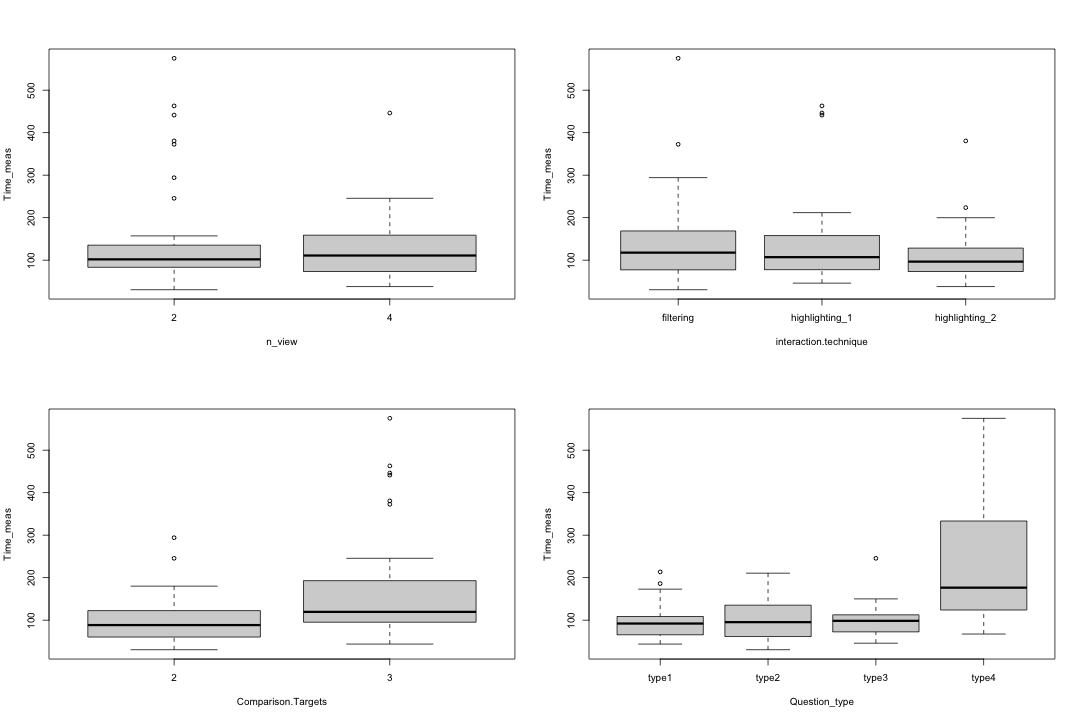
\includegraphics[width=15.5cm]{images/boxplots.png}


\subsection{Manipulating the distraction index}
Weil gesehen dass distraction index nicht gut korelliert, wir haben folgendes versucht

We decided to manipulate the distraction index in two ways and look how it impacts the results.
\begin{enumerate}
    \item Manipulating $\alpha$ of \ref{viewDistractionEquation}
    \item Manipulating $b_3$ of \ref{difficultyIndexEquation} (Distraction index as a whole)
\end{enumerate}




\section{Answer accuracy}

\subsection{Manipulating the discriminability index}